% !TEX root = ../../main.tex

\section{Vue 后台管理端核心模块实现}

Vue 后台管理端主要面向系统管理员，承担手势资源、样本数据、训练任务和模型版本等维护工作。
与移动端面向普通用户的训练识别流程不同，后台管理端更关注系统资源的可维护性和模型闭环的可管理性。
当前后台管理端基于 Vue 和 Element Plus 实现，通过统一请求封装访问 Spring Boot 服务端接口，并结合路由守卫和 token 机制完成后台访问控制。

后台管理端核心页面组织如图~\ref{fig:chapter05-admin-management-pages} 所示。

\begin{figure}[H]
  \centering
  \begin{subfigure}[t]{0.47\textwidth}
    \centering
    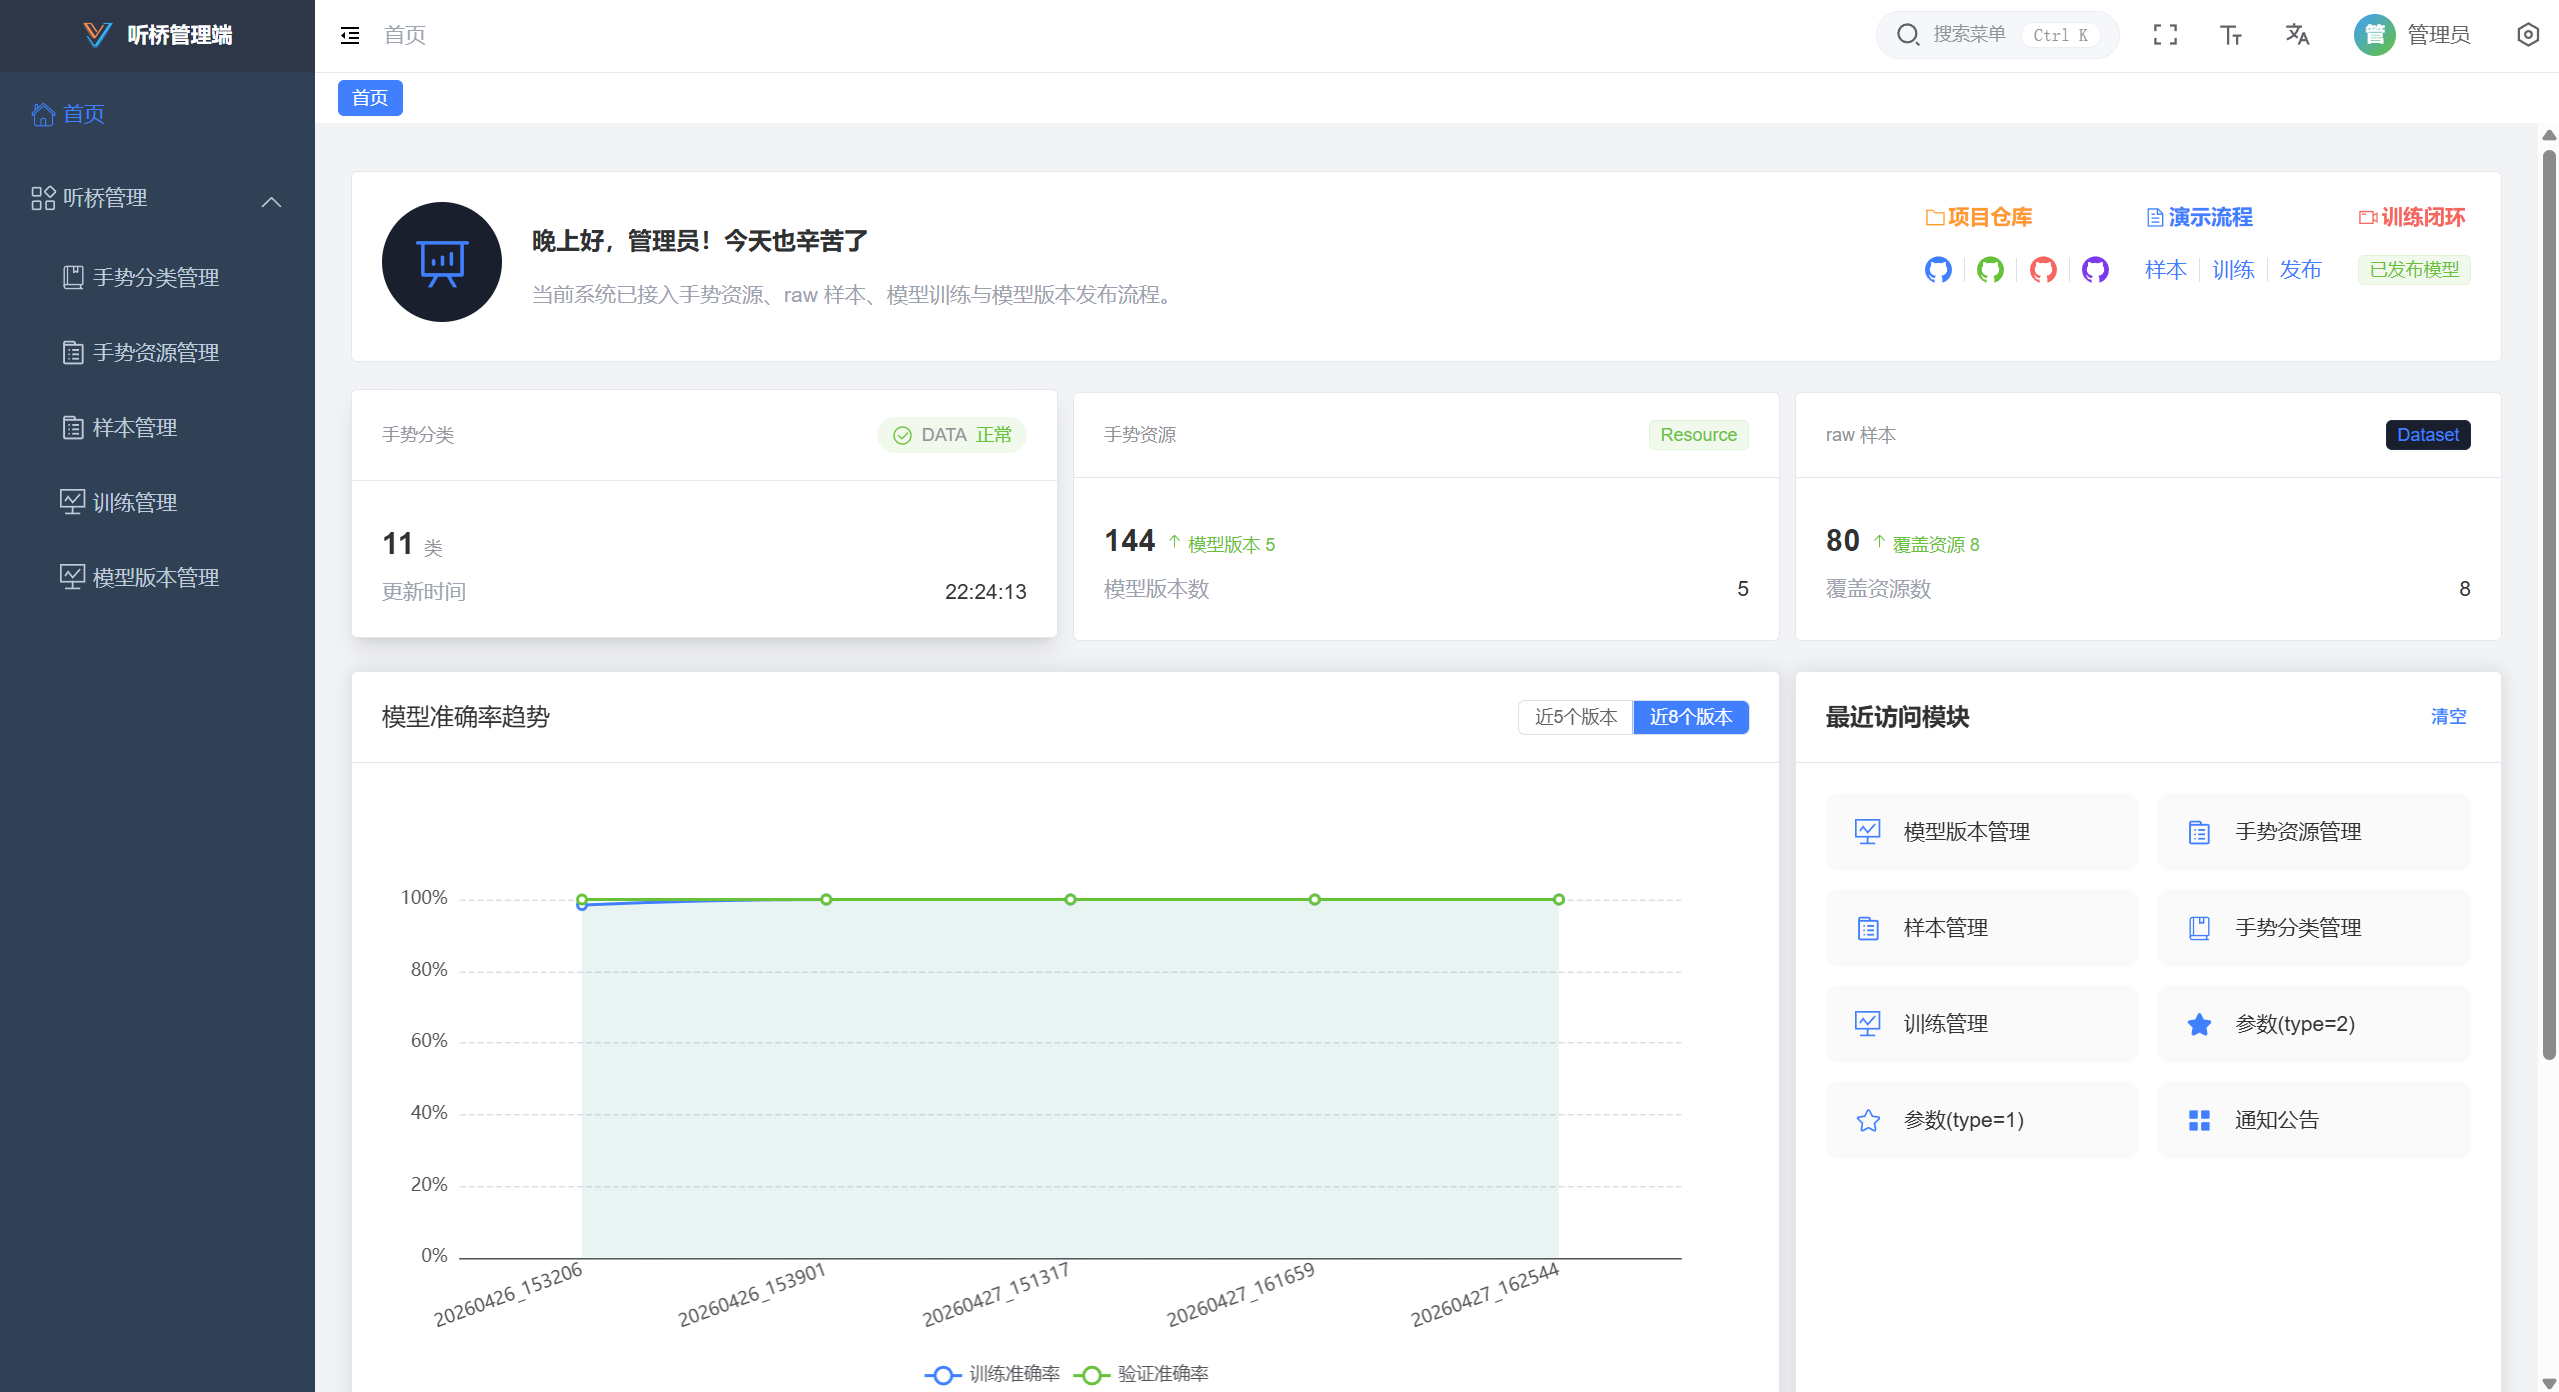
\includegraphics[width=\textwidth,height=0.23\textheight,keepaspectratio]{figures/chapter05/admin-system-overview.png}
    \caption{系统概览}
  \end{subfigure}
  \hfill
  \begin{subfigure}[t]{0.47\textwidth}
    \centering
    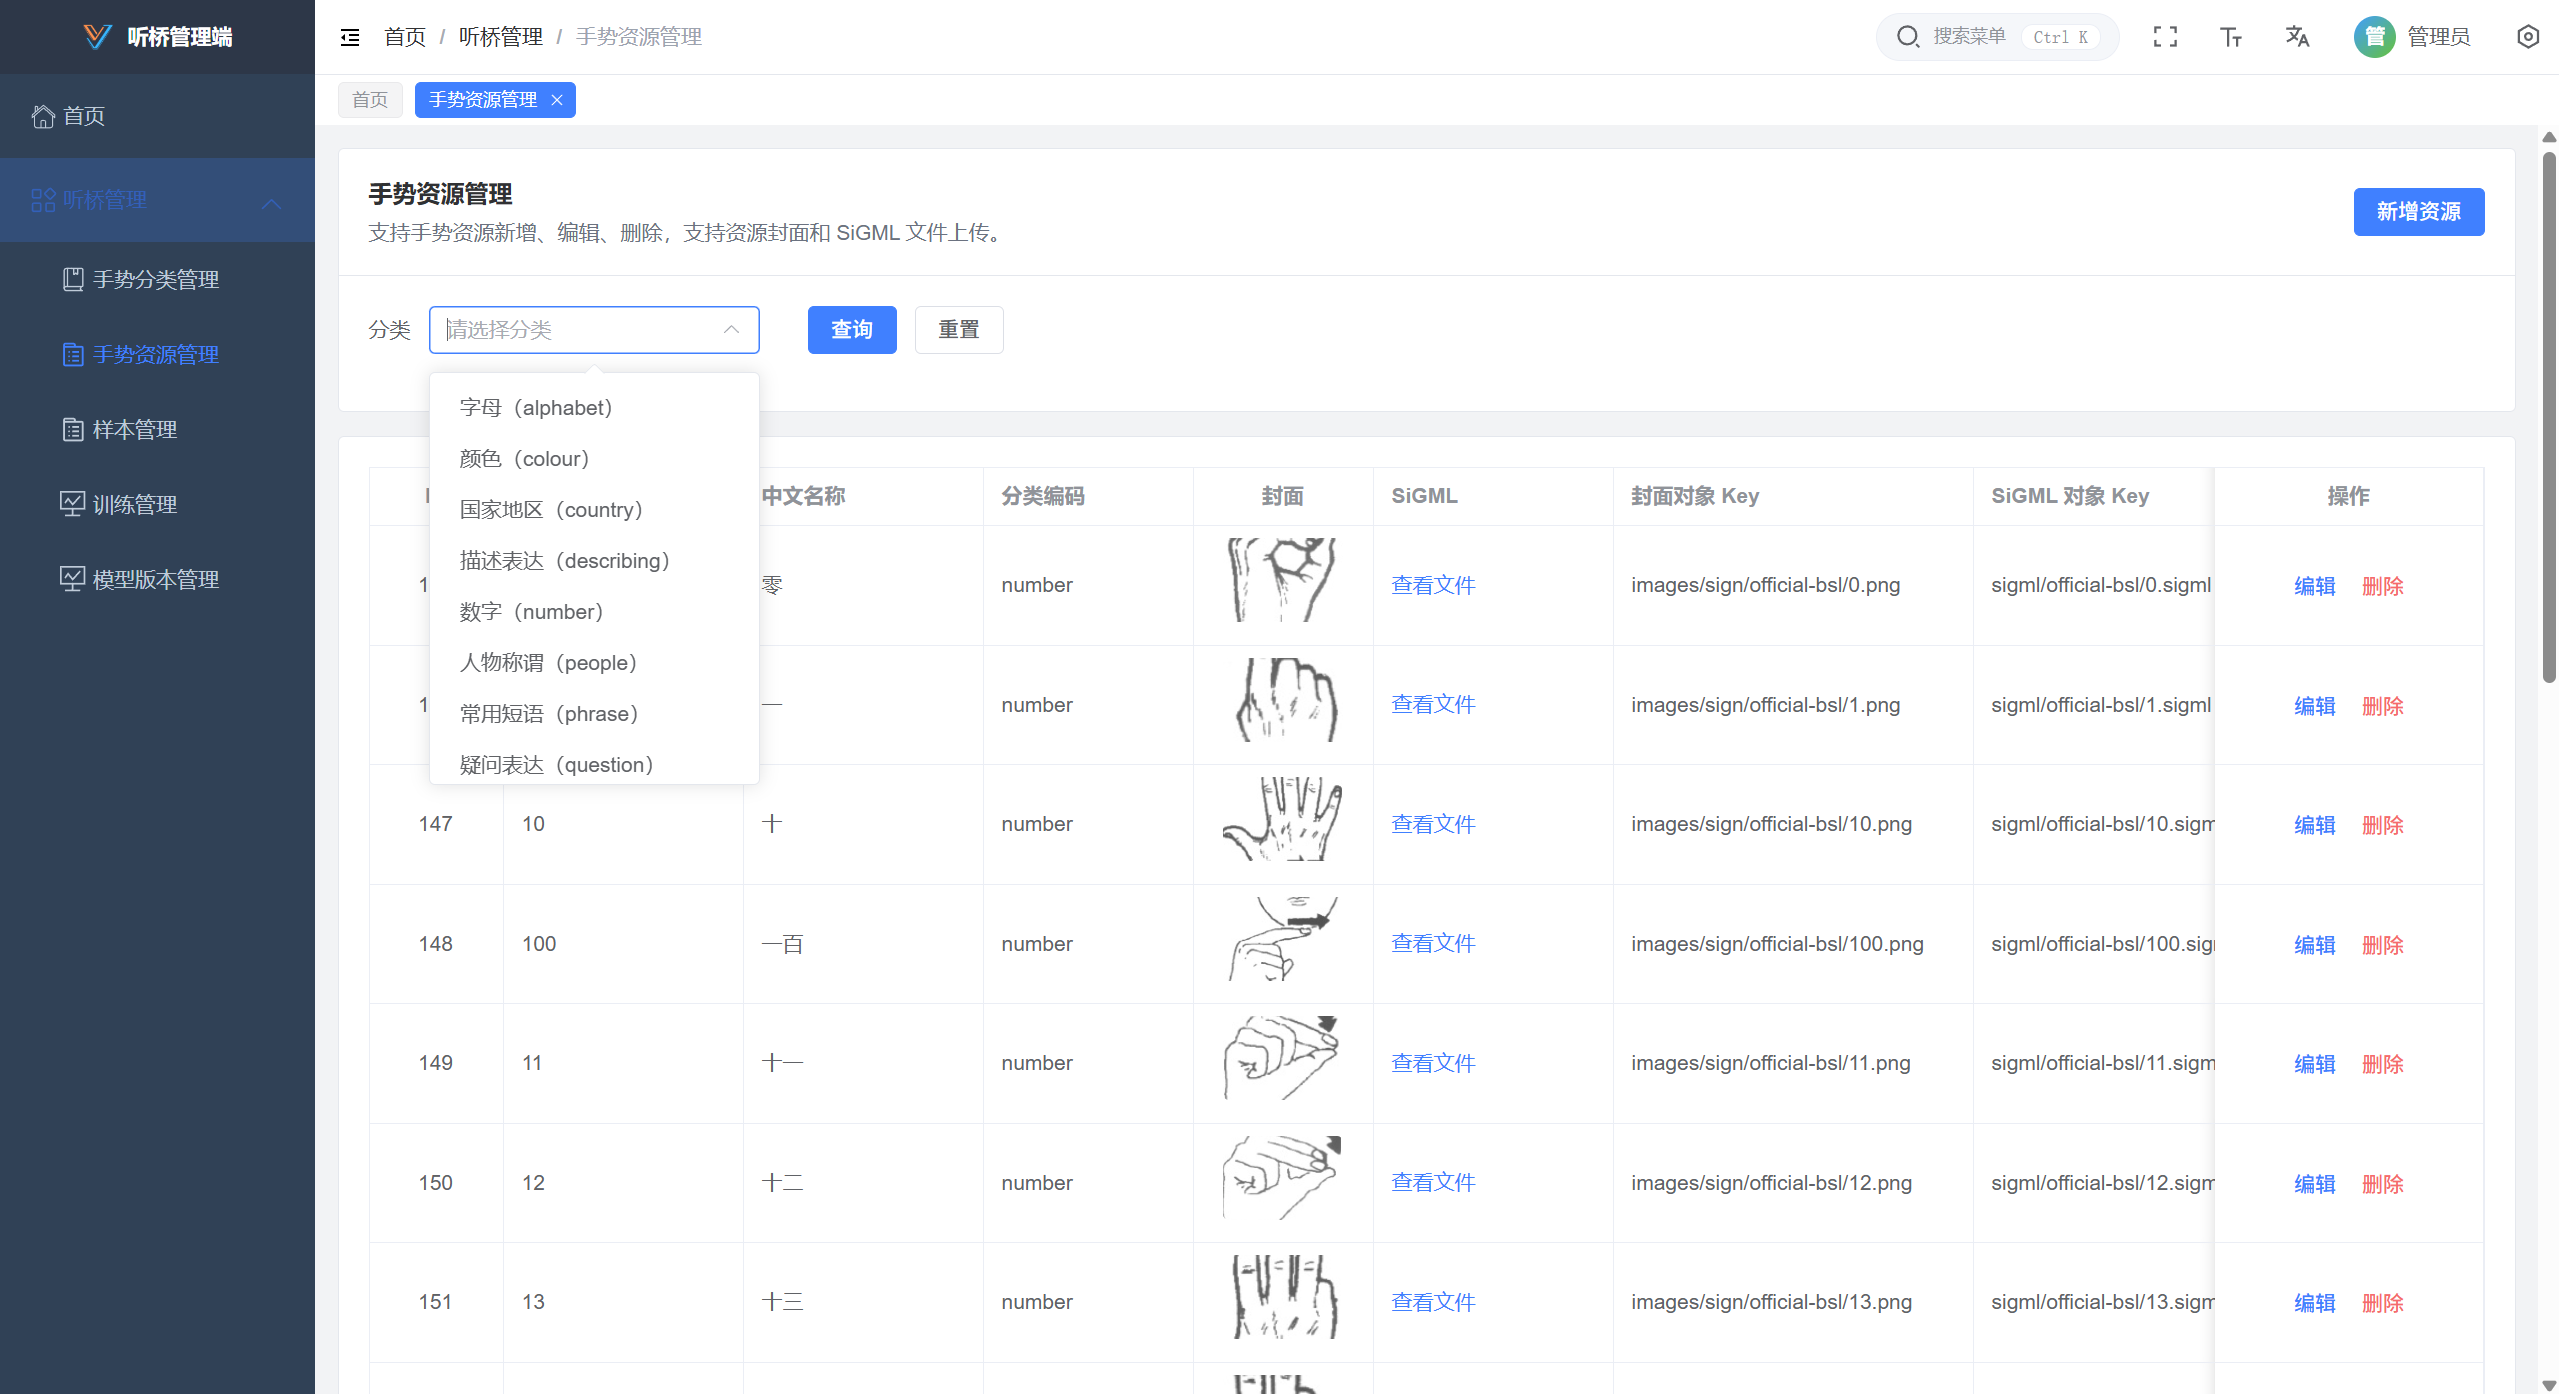
\includegraphics[width=\textwidth,height=0.23\textheight,keepaspectratio]{figures/chapter05/gesture-resource-management.png}
    \caption{手势资源管理}
  \end{subfigure}

  \vspace{6pt}

  \begin{subfigure}[t]{0.47\textwidth}
    \centering
    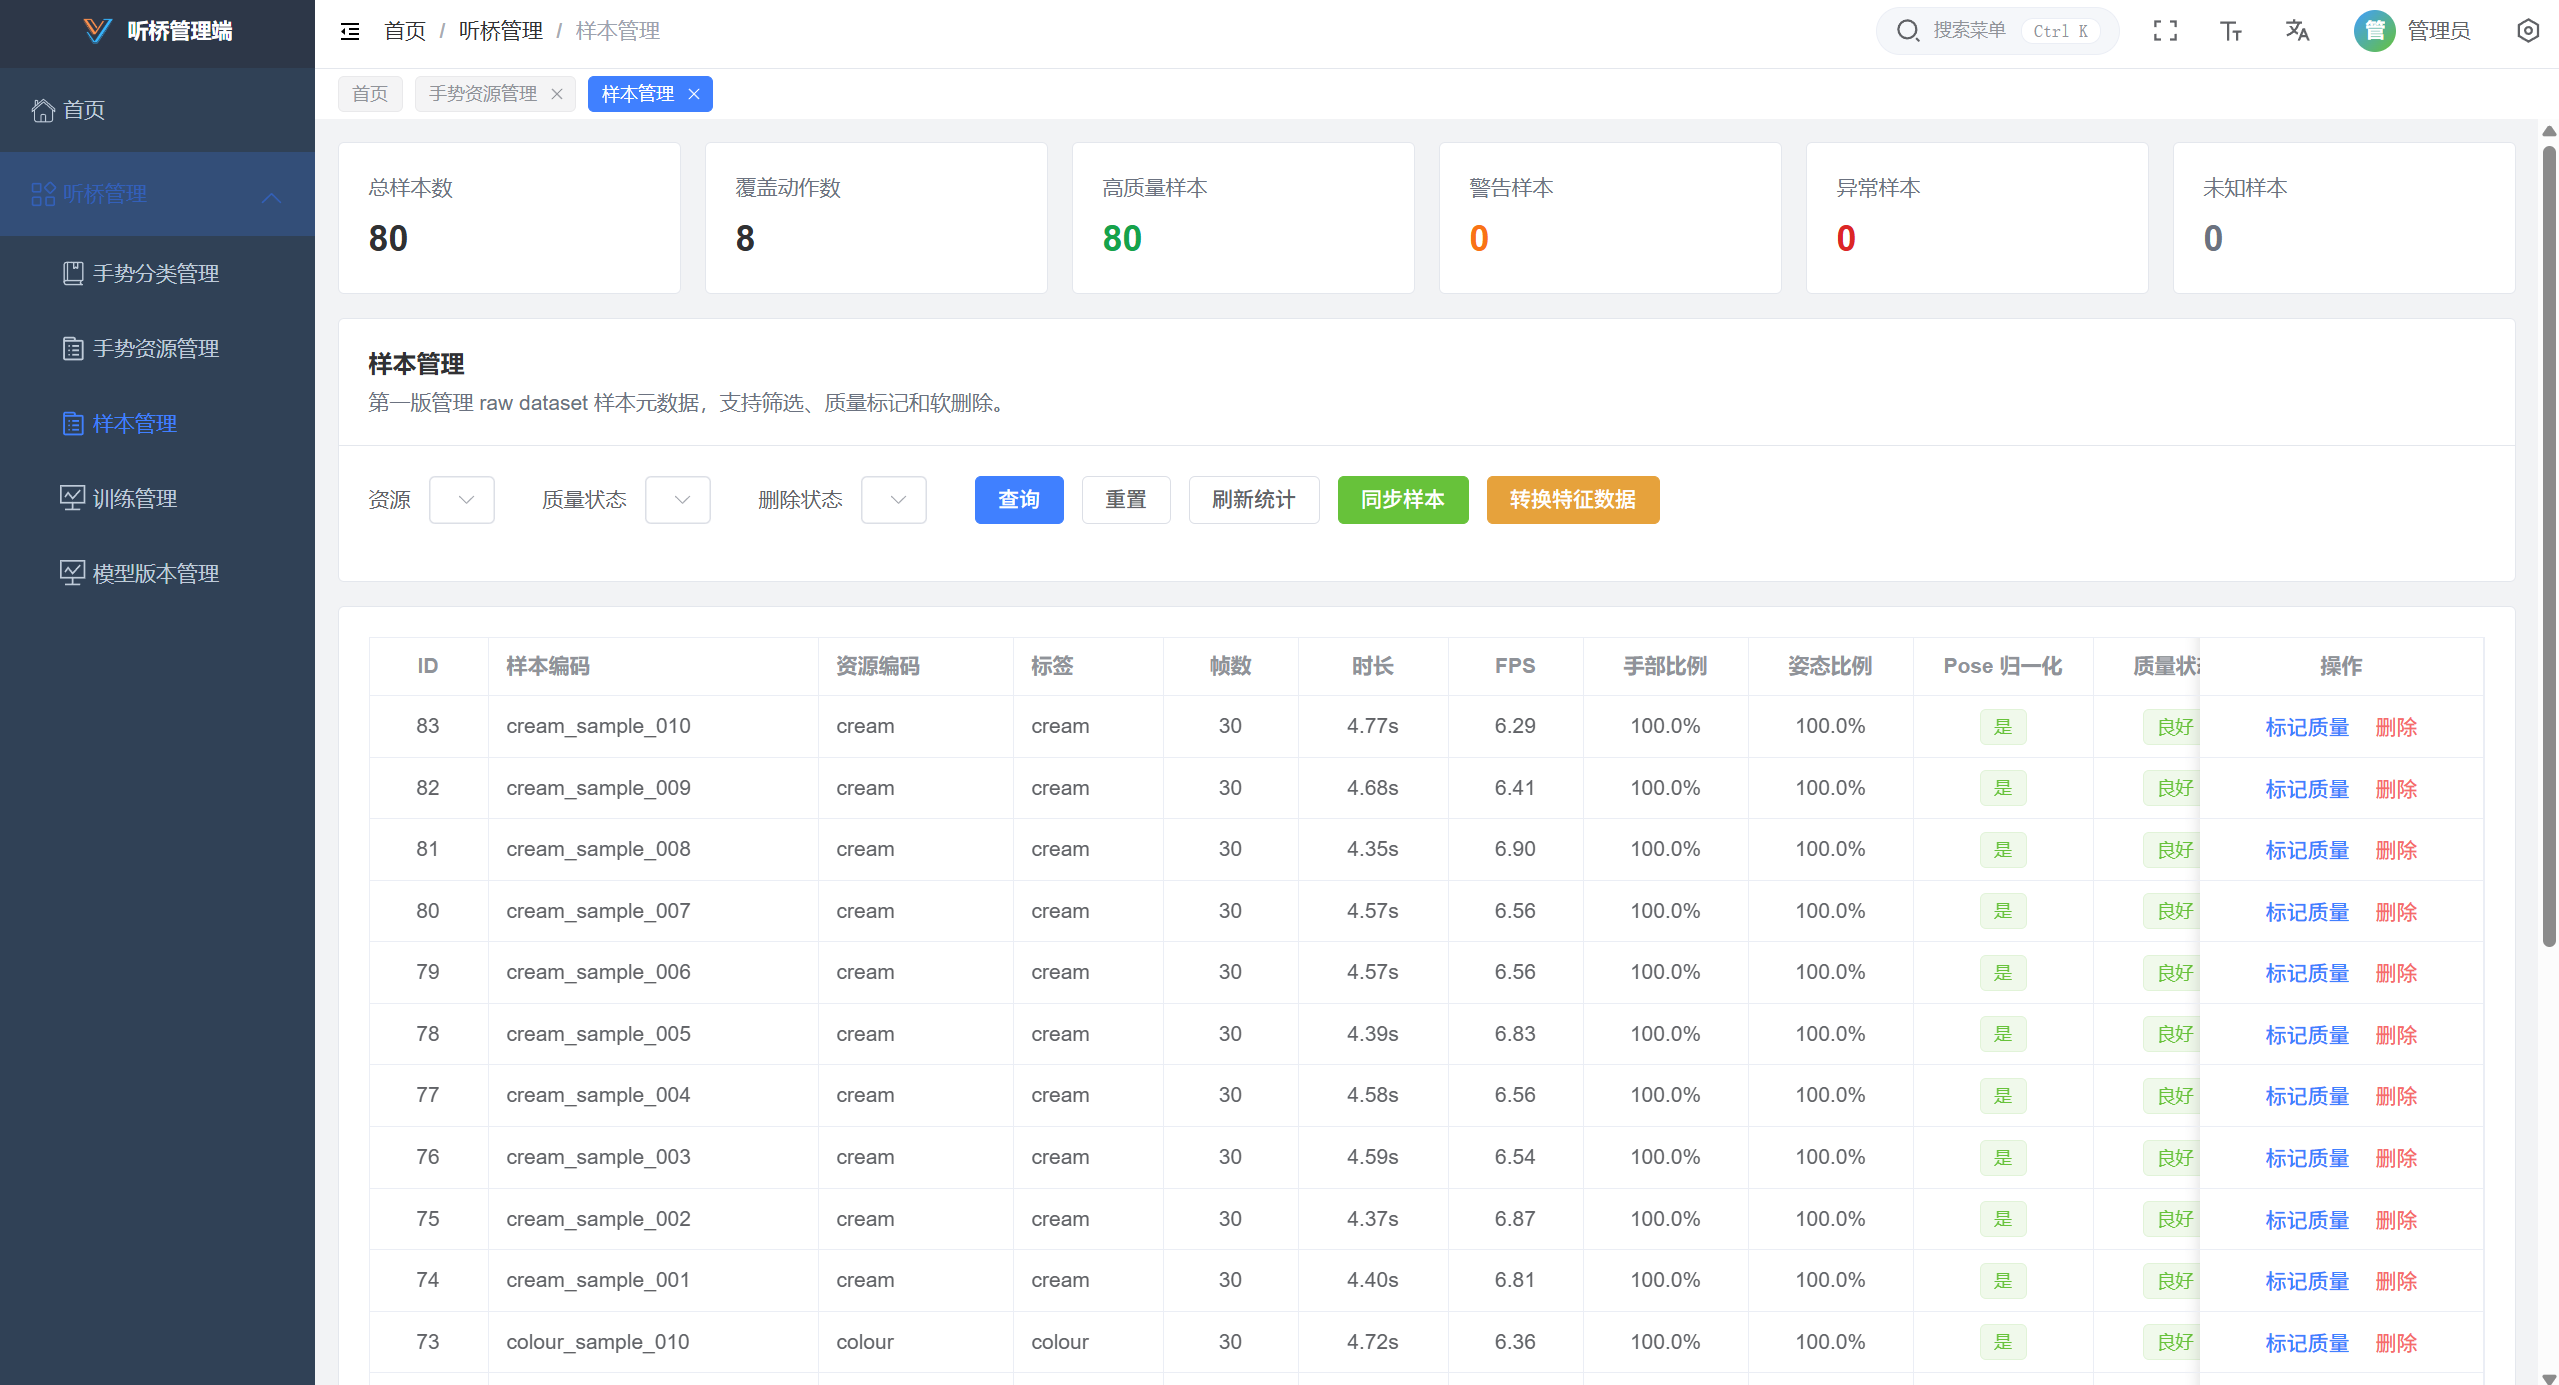
\includegraphics[width=\textwidth,height=0.23\textheight,keepaspectratio]{figures/chapter05/sample-management.png}
    \caption{样本管理}
  \end{subfigure}
  \hfill
  \begin{subfigure}[t]{0.47\textwidth}
    \centering
    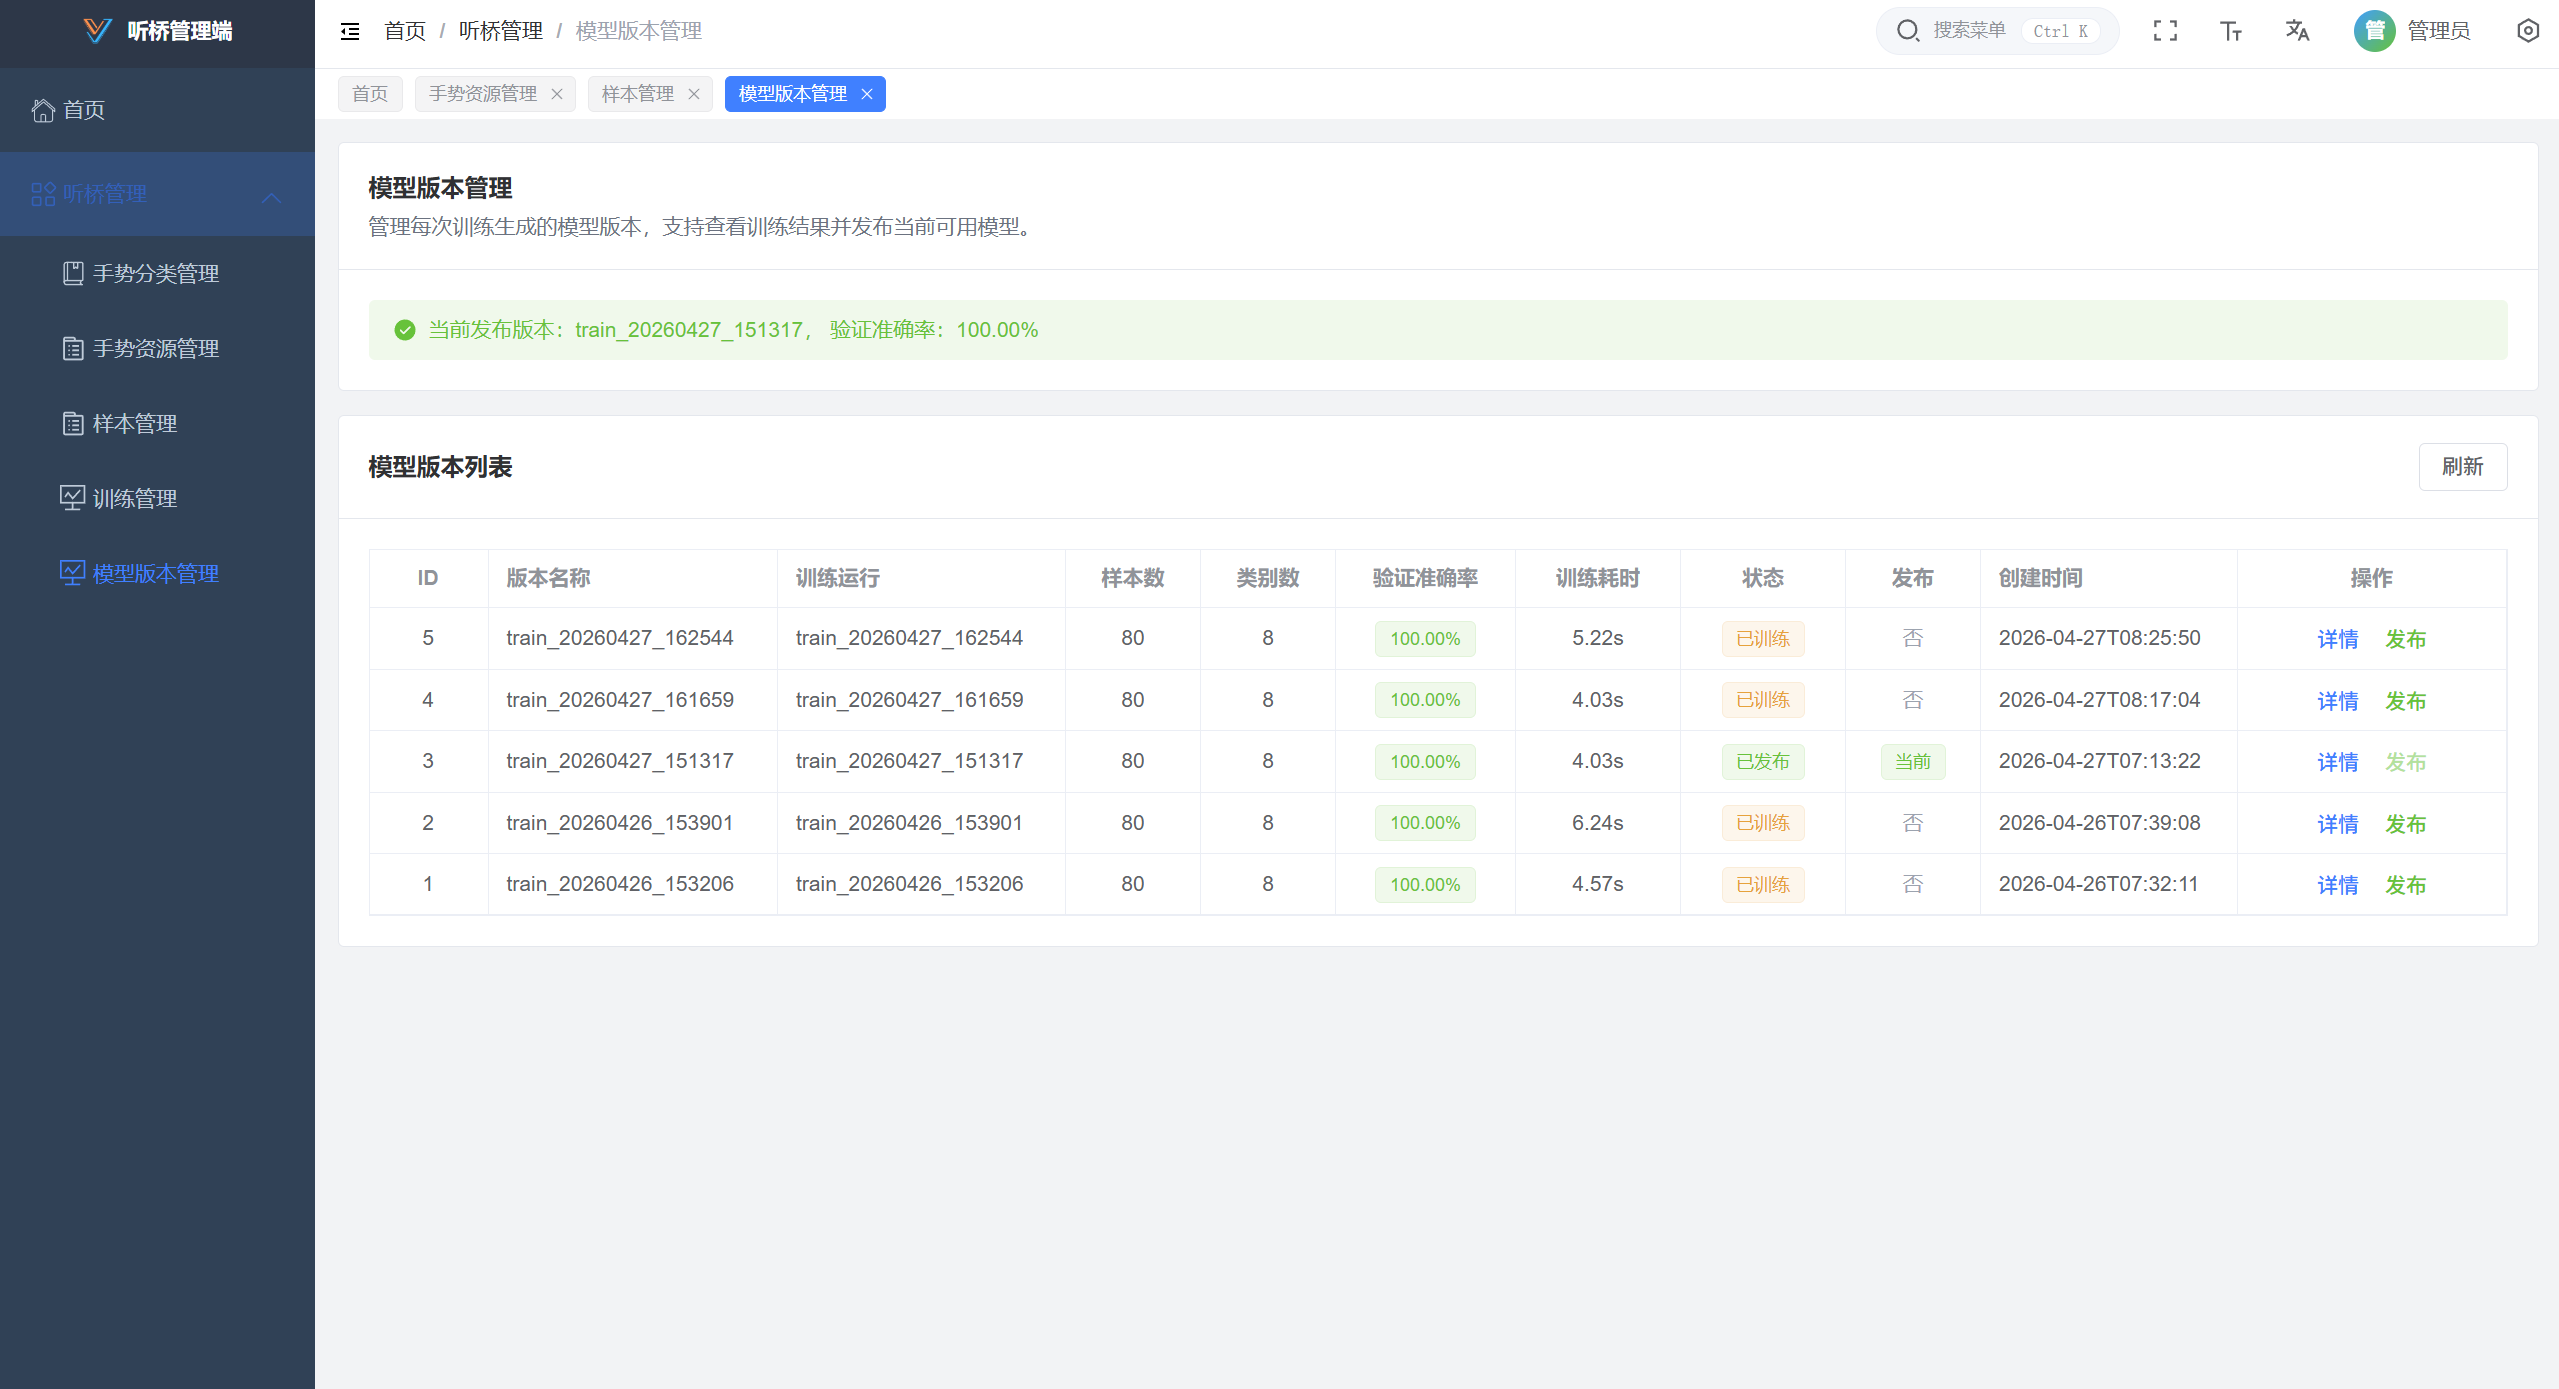
\includegraphics[width=\textwidth,height=0.23\textheight,keepaspectratio]{figures/chapter05/model-version-management.png}
    \caption{模型版本管理}
  \end{subfigure}

  \caption{后台管理端核心页面组织图}
  \label{fig:chapter05-admin-management-pages}
\end{figure}

后台管理端主要功能接口如表~\ref{tab:chapter05-admin-interfaces} 所示。

\WhuInterfaceTable{后台管理端主要功能接口}{tab:chapter05-admin-interfaces}{
登录认证 & POST & /admin/auth/login & 管理员登录并获取 token \\
系统概览 & GET & /admin/dashboard/overview & 获取资源、样本和模型概览数据 \\
分类管理 & GET/POST & /admin/sign/categories & 手势分类分页查询、新增和修改 \\
资源管理 & GET/POST & /admin/sign/resources & 手势资源分页查询、新增和修改 \\
样本管理 & GET/POST & /admin/sign/samples & 样本查询、删除和质量状态维护 \\
训练管理 & POST & /admin/training/start & 触发模型训练任务 \\
模型版本 & POST & /admin/model-versions/publish & 发布当前可用模型版本 \\
}

\subsection{登录认证与路由控制实现}

后台管理端首先实现管理员登录功能。
管理员输入账号和密码后，前端调用服务端登录接口，服务端校验通过后返回 token 和管理员基本信息。
前端将 token 保存到本地，并在后续请求中自动携带该 token。
若服务端返回登录失效或权限异常，前端会清理本地登录状态并跳转回登录页。

后台管理端采用基于路由的页面组织方式。
登录成功后进入后台主布局，主布局通常由侧边栏、顶部栏和内容区域组成。
侧边栏提供系统概览、手势分类管理、手势资源管理、样本管理、训练管理和模型版本管理等入口；
顶部栏用于展示当前管理员信息、退出登录和修改密码等操作；
内容区域根据当前路由展示具体业务页面。

路由守卫用于控制未登录用户访问后台页面。
当用户直接访问管理端内部路由时，前端会先判断本地是否存在有效 token，若不存在则跳转到登录页。
通过这种方式，后台管理端在前端层面实现了基本访问保护，同时服务端仍会在接口层面进行 token 校验，避免仅依赖前端控制。

此外，后台管理端还需要处理 token 过期、退出登录和修改密码等状态变化。
当接口返回登录失效状态时，前端应清除本地 token 和管理员信息，并引导用户重新登录。
通过登录认证和路由控制的结合，后台管理端能够形成较完整的访问控制流程。

\subsection{手势分类与手势资源管理实现}

手势分类管理用于维护移动端资源展示的分类基础。
管理员可以在后台新增、修改、删除或启用禁用分类。
分类信息通常包括分类名称、分类编码、排序值和状态等字段。
前端页面通过表格展示分类列表，并提供新增、编辑和删除等操作入口。
管理员提交表单后，前端调用服务端接口完成数据更新。

手势资源管理是后台管理端的核心功能之一。
管理员可以维护每个手势资源的资源编码、资源名称、所属分类、封面资源、动作示范资源和启用状态等信息。
资源编码与识别服务中的标签体系存在对应关系，因此在资源维护时需要保证资源编码具有稳定性，避免移动端训练资源与模型输出标签之间产生不一致。

在页面实现上，手势资源管理通常采用“查询表格 + 编辑弹窗 + 文件上传”的形式。
表格用于展示资源列表，筛选条件用于按名称、分类或状态查询资源；
编辑弹窗用于填写资源字段；
文件上传组件用于上传封面或动作示范资源。
上传成功后，前端将文件地址与资源表单一起提交给服务端，由服务端保存资源元数据和文件访问路径。

通过分类管理和资源管理，后台管理员可以在不修改移动端代码的情况下扩充或调整训练内容。
移动端通过接口读取已启用的分类和资源，从而动态展示最新训练内容。
这种实现方式使系统内容维护与用户端展示相互解耦，提高了资源管理效率。

\subsection{样本管理与模型训练管理实现}

样本管理用于查看和维护手势识别训练所需的数据。
样本数据通常与具体手势资源关联，后台页面需要展示样本所属标签、样本文件地址、样本质量状态、样本来源和样本状态等信息。
管理员可以查看样本列表，筛选某个手势资源下的样本，也可以删除明显错误或质量较差的样本。

样本管理的意义在于为模型训练提供可控的数据基础。
由于手势识别效果高度依赖训练样本质量，系统需要为管理员提供样本查看和筛选能力。
对于采集到的低质量样本，管理员可以通过后台进行删除或标记，从而减少其对后续模型训练的影响。

模型训练管理用于触发或查看模型训练相关任务。
后台管理端向服务端发送训练请求，由服务端进一步调用 Python 手势识别服务完成特征转换和模型训练。
训练完成后，Python 服务或服务端将训练结果保存为模型文件、标签映射文件和评估指标，再由服务端登记为模型版本。
后台管理端负责展示训练状态和训练结果，使管理员能够了解模型训练是否成功以及模型效果是否满足发布条件。

在当前系统实现中，样本管理、模型训练管理和模型版本管理共同构成识别能力更新闭环。
样本管理提供数据基础，模型训练管理生成模型产物，模型版本管理负责登记和发布模型。
通过该闭环，系统能够在新增样本或扩充动作类别后重新训练模型，并将新模型发布到识别服务中。

\subsection{模型版本管理实现}

模型版本管理用于维护识别模型的版本信息和发布状态。
每个模型版本通常包含版本名称、模型文件地址、标签映射文件地址、支持动作数量、训练样本数量、准确率和发布状态等信息。
管理员可以在后台查看所有模型版本，并选择某个版本进行发布。

在页面实现上，模型版本管理通常以表格形式展示版本名称、支持动作数量、样本数量、准确率、创建时间和发布状态等信息。
管理员可以根据模型版本状态判断当前模型是否可用，也可以通过发布操作将指定模型设置为当前识别服务使用的模型。

模型版本管理需要与样本管理、训练管理和 Python 识别服务保持联动。
训练完成后生成的模型文件和标签映射文件需要登记为模型版本；
管理员发布某一模型版本后，服务端需要更新版本状态，并通知 Python 识别服务加载对应模型。
通过这种方式，后台管理端能够对模型迭代过程进行统一管理。

系统概览页面可以辅助管理员查看资源数量、样本数量、模型版本状态和当前发布模型等信息，但其主要作用是提供全局状态摘要。
模型版本管理本身更关注模型版本数据维护、发布状态控制和识别服务联动，是后台管理端模型维护闭环中的关键模块。
